% Asset ID: FAS1ConicSections1TikZ-004
% Source: FP1-Chp2-ConicSections1.pdf tangent/normal evidence
% Purpose: Show the tangent and normal at P(at^2,2at) on y^2 = 4ax.
\documentclass[tikz,border=6pt]{standalone}
\usepackage{amsmath}
\usepackage{xcolor}
\usetikzlibrary{arrows.meta,calc,backgrounds}
\definecolor{canvas}{HTML}{FAF9F6}
\definecolor{ivory}{HTML}{FFFFF0}
\definecolor{linegray}{HTML}{E5E5EA}
\definecolor{gold}{HTML}{C5A059}
\definecolor{ink}{HTML}{2C2C2E}
\definecolor{rose}{HTML}{FBEFEF}
\definecolor{teal}{HTML}{6B9FA3}
\definecolor{purple}{HTML}{8F6C9F}
\begin{document}
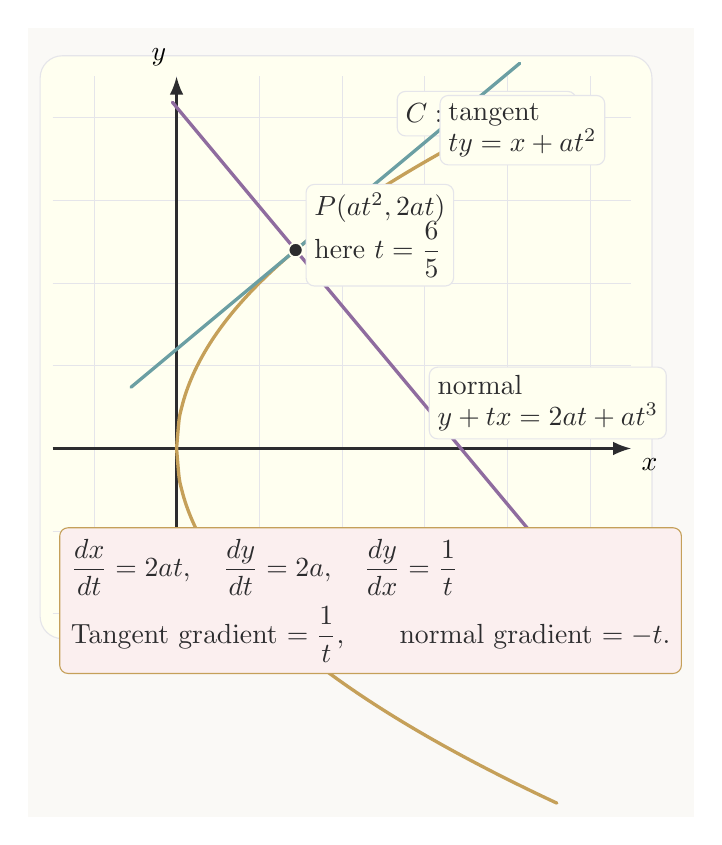
\begin{tikzpicture}[x=1.05cm,y=1.05cm,>=Latex,background rectangle/.style={fill=canvas},show background rectangle,
axis/.style={->,thick,draw=ink},gridline/.style={draw=linegray,line width=0.25pt},curve/.style={draw=gold,very thick,line cap=round},tangent/.style={draw=teal,very thick,line cap=round},normal/.style={draw=purple,very thick,line cap=round},point/.style={circle,fill=ink,draw=ivory,line width=0.6pt,inner sep=1.8pt},labelbox/.style={fill=ivory,draw=linegray,rounded corners=3pt,inner sep=3pt,align=left,text=ink},resultbox/.style={fill=rose,draw=gold,rounded corners=3pt,inner sep=4pt,align=left,text=ink}]
\pgfmathsetmacro{\tval}{1.2}
\pgfmathsetmacro{\px}{\tval*\tval}
\pgfmathsetmacro{\py}{2*\tval}
\pgfmathsetmacro{\normalintercept}{2*\tval+\tval*\tval*\tval}
\fill[ivory,rounded corners=8pt,draw=linegray] (-1.65,-2.3) rectangle (5.75,4.75);
\foreach \x in {-1,0,...,5}{\draw[gridline] (\x,-2)--(\x,4.5);}
\foreach \y in {-2,-1,...,4}{\draw[gridline] (-1.5,\y)--(5.5,\y);}
\draw[axis] (-1.5,0)--(5.5,0) node[below right] {$x$};
\draw[axis] (0,-2)--(0,4.5) node[above left] {$y$};
\draw[curve,domain=0:4.6,samples=150,smooth,variable=\x] plot ({\x},{2*sqrt(\x)});
\draw[curve,domain=0:4.6,samples=150,smooth,variable=\x] plot ({\x},{-2*sqrt(\x)});
\node[labelbox] at (3.75,4.05) {$C:\ y^2=4ax$};
\draw[tangent,domain=-0.55:4.15,samples=2,variable=\x] plot ({\x},{(\x+\tval*\tval)/\tval});
\draw[normal,domain=-0.05:4.55,samples=2,variable=\x] plot ({\x},{-\tval*\x+\normalintercept});
\coordinate (P) at (\px,\py);
\node[point] at (P) {};
\node[labelbox,anchor=west] at ($(P)+(0.12,0.18)$) {$P(at^2,2at)$\\[-1pt] here $t=\dfrac65$};
\node[labelbox,anchor=west] at (3.18,3.85) {tangent\\[-1pt] $ty=x+at^2$};
\node[labelbox,anchor=west] at (3.05,0.55) {normal\\[-1pt] $y+tx=2at+at^3$};
\node[resultbox,anchor=west] at (-1.42,-1.84) {$\dfrac{dx}{dt}=2at,\quad \dfrac{dy}{dt}=2a,\quad\dfrac{dy}{dx}=\dfrac{1}{t}$\\[3pt] Tangent gradient $=\dfrac1t$,\qquad normal gradient $=-t$.};
\end{tikzpicture}
\end{document}
